% Options for packages loaded elsewhere
% Options for packages loaded elsewhere
\PassOptionsToPackage{unicode}{hyperref}
\PassOptionsToPackage{hyphens}{url}
\PassOptionsToPackage{dvipsnames,svgnames,x11names}{xcolor}
%
\documentclass[
  12pt,
  oneside,
  a4paper,
  english,
  brazil]{abntex2}
\usepackage{xcolor}
\usepackage[top=30mm,left=30mm,right=20mm,bottom=20mm]{geometry}
\usepackage{amsmath,amssymb}
\setcounter{secnumdepth}{5}
\usepackage{iftex}
\ifPDFTeX
  \usepackage[T1]{fontenc}
  \usepackage[utf8]{inputenc}
  \usepackage{textcomp} % provide euro and other symbols
\else % if luatex or xetex
  \usepackage{unicode-math} % this also loads fontspec
  \defaultfontfeatures{Scale=MatchLowercase}
  \defaultfontfeatures[\rmfamily]{Ligatures=TeX,Scale=1}
\fi
\usepackage{lmodern}
\ifPDFTeX\else
  % xetex/luatex font selection
\fi
% Use upquote if available, for straight quotes in verbatim environments
\IfFileExists{upquote.sty}{\usepackage{upquote}}{}
\IfFileExists{microtype.sty}{% use microtype if available
  \usepackage[]{microtype}
  \UseMicrotypeSet[protrusion]{basicmath} % disable protrusion for tt fonts
}{}
\makeatletter
\@ifundefined{KOMAClassName}{% if non-KOMA class
  \IfFileExists{parskip.sty}{%
    \usepackage{parskip}
  }{% else
    \setlength{\parindent}{0pt}
    \setlength{\parskip}{6pt plus 2pt minus 1pt}}
}{% if KOMA class
  \KOMAoptions{parskip=half}}
\makeatother
% Make \paragraph and \subparagraph free-standing
\makeatletter
\ifx\paragraph\undefined\else
  \let\oldparagraph\paragraph
  \renewcommand{\paragraph}{
    \@ifstar
      \xxxParagraphStar
      \xxxParagraphNoStar
  }
  \newcommand{\xxxParagraphStar}[1]{\oldparagraph*{#1}\mbox{}}
  \newcommand{\xxxParagraphNoStar}[1]{\oldparagraph{#1}\mbox{}}
\fi
\ifx\subparagraph\undefined\else
  \let\oldsubparagraph\subparagraph
  \renewcommand{\subparagraph}{
    \@ifstar
      \xxxSubParagraphStar
      \xxxSubParagraphNoStar
  }
  \newcommand{\xxxSubParagraphStar}[1]{\oldsubparagraph*{#1}\mbox{}}
  \newcommand{\xxxSubParagraphNoStar}[1]{\oldsubparagraph{#1}\mbox{}}
\fi
\makeatother


\usepackage{longtable,booktabs,array}
\usepackage{calc} % for calculating minipage widths
% Correct order of tables after \paragraph or \subparagraph
\usepackage{etoolbox}
\makeatletter
\patchcmd\longtable{\par}{\if@noskipsec\mbox{}\fi\par}{}{}
\makeatother
% Allow footnotes in longtable head/foot
\IfFileExists{footnotehyper.sty}{\usepackage{footnotehyper}}{\usepackage{footnote}}
\makesavenoteenv{longtable}
\usepackage{graphicx}
\makeatletter
\newsavebox\pandoc@box
\newcommand*\pandocbounded[1]{% scales image to fit in text height/width
  \sbox\pandoc@box{#1}%
  \Gscale@div\@tempa{\textheight}{\dimexpr\ht\pandoc@box+\dp\pandoc@box\relax}%
  \Gscale@div\@tempb{\linewidth}{\wd\pandoc@box}%
  \ifdim\@tempb\p@<\@tempa\p@\let\@tempa\@tempb\fi% select the smaller of both
  \ifdim\@tempa\p@<\p@\scalebox{\@tempa}{\usebox\pandoc@box}%
  \else\usebox{\pandoc@box}%
  \fi%
}
% Set default figure placement to htbp
\def\fps@figure{htbp}
\makeatother


% definitions for citeproc citations
\NewDocumentCommand\citeproctext{}{}
\NewDocumentCommand\citeproc{mm}{%
  \begingroup\def\citeproctext{#2}\cite{#1}\endgroup}
\makeatletter
 % allow citations to break across lines
 \let\@cite@ofmt\@firstofone
 % avoid brackets around text for \cite:
 \def\@biblabel#1{}
 \def\@cite#1#2{{#1\if@tempswa , #2\fi}}
\makeatother
\newlength{\cslhangindent}
\setlength{\cslhangindent}{1.5em}
\newlength{\csllabelwidth}
\setlength{\csllabelwidth}{3em}
\newenvironment{CSLReferences}[2] % #1 hanging-indent, #2 entry-spacing
 {\begin{list}{}{%
  \setlength{\itemindent}{0pt}
  \setlength{\leftmargin}{0pt}
  \setlength{\parsep}{0pt}
  % turn on hanging indent if param 1 is 1
  \ifodd #1
   \setlength{\leftmargin}{\cslhangindent}
   \setlength{\itemindent}{-1\cslhangindent}
  \fi
  % set entry spacing
  \setlength{\itemsep}{#2\baselineskip}}}
 {\end{list}}
\usepackage{calc}
\newcommand{\CSLBlock}[1]{\hfill\break\parbox[t]{\linewidth}{\strut\ignorespaces#1\strut}}
\newcommand{\CSLLeftMargin}[1]{\parbox[t]{\csllabelwidth}{\strut#1\strut}}
\newcommand{\CSLRightInline}[1]{\parbox[t]{\linewidth - \csllabelwidth}{\strut#1\strut}}
\newcommand{\CSLIndent}[1]{\hspace{\cslhangindent}#1}



\setlength{\emergencystretch}{3em} % prevent overfull lines

\providecommand{\tightlist}{%
  \setlength{\itemsep}{0pt}\setlength{\parskip}{0pt}}



 


% ---
% Pacotes básicos 
% ---
\usepackage{lmodern}			% Usa a fonte Latin Modern			
\usepackage[T1]{fontenc}		% Selecao de codigos de fonte.
\usepackage[utf8]{inputenc}		% Codificacao do documento (conversão automática dos acentos)
\usepackage{lastpage}			% Usado pela Ficha catalográfica
\usepackage{indentfirst}		% Indenta o primeiro parágrafo de cada seção.
\usepackage{color}				% Controle das cores
\usepackage{graphicx}			% Inclusão de gráficos
\usepackage{microtype} 			% para melhorias de justificação
\usepackage{amsmath}
\usepackage{amssymb}
\usepackage{upgreek}
\usepackage{listings}			% Inclusão de código fonte 			


% Pacotes de citações
% ---
% \usepackage[brazilian,hyperpageref]{backref}	 % Paginas com as citações na bibl

% --- 
% CONFIGURAÇÕES DE PACOTES
% --- 

% ---
% Configurações de aparência do PDF final

% alterando o aspecto da cor azul
\definecolor{blue}{RGB}{41,5,195}

% informações do PDF
\makeatletter
\hypersetup{
     	%pagebackref=true,
		% pdftitle={\@title}, 
		% pdfauthor={\@author},
    	% pdfsubject={\imprimirpreambulo},
	    % pdfcreator={LaTeX with abnTeX2},
		% pdfkeywords={abnt}{latex}{abntex}{abntex2}{trabalho acadêmico}, 
		colorlinks=true,       		% false: boxed links; true: colored links
    	linkcolor=blue,          	% color of internal links
    	citecolor=blue,        		% color of links to bibliography
    	filecolor=magenta,      		% color of file links
		urlcolor=blue,
		bookmarksdepth=4
}

% Comandos de uso do orientador para sugestão de alterações:
\usepackage{xcolor}
\usepackage{cancel}

\colorlet{oliveGreen}{blue!20!black!50!green}

\usepackage{soul}
\usepackage{soulutf8}
\setstcolor{red}

\newcommand{\cito}[1]{\textsuperscript{\cite{#1}}} % numeração da citação sobreescrita
\newcommand{\PROFESSOR}[1]{\textcolor{red}{\MakeUppercase{#1}}} % Acrescenta um nota pelo professor
\newcommand{\PROFESSORDEL}[1]{\textcolor{red}{\st{#1}}} % removido pelo professor
\newcommand{\PROFESSORADD}[1]{\textcolor{oliveGreen}{#1}} % adicionado pelo professor
\newcommand{\PROFESSORREP}[2]{\PROFESSORDEL{#1}\PROFESSORADD{#2}} % substituir


\renewcommand{\printtoctitle}[1]{\normalsize\bfseries\centering TABLE OF CONTENTS}


% Adiciona indentação para seções e subseções no sumário
\cftsetindents{chapter}{0em}{0em}
\cftsetindents{section}{1.5em}{2.5em}
\cftsetindents{subsection}{3em}{3.5em}
\cftsetindents{subsubsection}{4.5em}{5em}

\AtBeginDocument{\captionsetup{labelfont=bf}}


\makeatother
% --- 

% --- 
% Espaçamentos entre linhas e parágrafos 
% --- 

% O tamanho do parágrafo é dado por:
\setlength{\parindent}{1.3cm}

% Controle do espaçamento entre um parágrafo e outro:
\setlength{\parskip}{0.2cm}  % tente também \onelineskip

% ---
% compila o indice
% ---
\makeindex
% ---
\makeatletter
\@ifpackageloaded{caption}{}{\usepackage{caption}}
\AtBeginDocument{%
\ifdefined\contentsname
  \renewcommand*\contentsname{Table of contents}
\else
  \newcommand\contentsname{Table of contents}
\fi
\ifdefined\listfigurename
  \renewcommand*\listfigurename{List of Figures}
\else
  \newcommand\listfigurename{List of Figures}
\fi
\ifdefined\listtablename
  \renewcommand*\listtablename{List of Tables}
\else
  \newcommand\listtablename{List of Tables}
\fi
\ifdefined\figurename
  \renewcommand*\figurename{Figure}
\else
  \newcommand\figurename{Figure}
\fi
\ifdefined\tablename
  \renewcommand*\tablename{Table}
\else
  \newcommand\tablename{Table}
\fi
}
\@ifpackageloaded{float}{}{\usepackage{float}}
\floatstyle{ruled}
\@ifundefined{c@chapter}{\newfloat{codelisting}{h}{lop}}{\newfloat{codelisting}{h}{lop}[chapter]}
\floatname{codelisting}{Code}
\newcommand*\listoflistings{\listof{codelisting}{List of Code}}
\makeatother
\makeatletter
\makeatother
\makeatletter
\@ifpackageloaded{caption}{}{\usepackage{caption}}
\@ifpackageloaded{subcaption}{}{\usepackage{subcaption}}
\makeatother
\makeatletter
\@ifpackageloaded{tcolorbox}{}{\usepackage[skins,breakable]{tcolorbox}}
\makeatother
\makeatletter
\@ifundefined{shadecolor}{\definecolor{shadecolor}{rgb}{.97, .97, .97}}{}
\makeatother
\makeatletter
\makeatother
\makeatletter
\ifdefined\Shaded\renewenvironment{Shaded}{\begin{tcolorbox}[breakable, borderline west={3pt}{0pt}{shadecolor}, interior hidden, enhanced, sharp corners, frame hidden, boxrule=0pt]}{\end{tcolorbox}}\fi
\makeatother
\usepackage{bookmark}
\IfFileExists{xurl.sty}{\usepackage{xurl}}{} % add URL line breaks if available
\urlstyle{same}
\hypersetup{
  colorlinks=true,
  linkcolor={blue},
  filecolor={Maroon},
  citecolor={Blue},
  urlcolor={Blue},
  pdfcreator={LaTeX via pandoc}}


\author{}
\date{}
\begin{document}


\setlength{\parindent}{0mm}
\ABNTEXchapterfont\normalsize

\ABNTEXchapterfont\normalsize

\begin{center}
\Large{\textbf{\uppercase{ Instituto Tecnológico de Aeronáutica }}}

\vspace{1cm}

\begin{figure}[H]
\centering


\includegraphics[width=0.6\textwidth]{figuras/ITA_logo.png}

\end{figure}

\vspace{2cm}

\large{\textbf{ Brian Clark Zanfelice }}

\vspace{1cm}

\Large{\textbf{\uppercase{ Methodology for Developing a Level 1 Digital Twin with AI Integration for Gas Turbines }}}

\vspace{3cm}

Final Paper

2025

\vfill

\huge{\textbf{ Course of Mechanical Aeronautics Engineering }}


\end{center}

\newpage{}

\vspace*{\fill}

\hfill
\begin{minipage}{0.90\textwidth}
    \begin{flushright}
        \textit{ "No que diz respeito ao empenho, ao compromisso, ao esforço, à dedicação, não existe meio-termo. Ou você faz uma coisa bem-feita ou não faz." } \\
        \textit{ AYRTON SENNA }
    \end{flushright}
\end{minipage}

\vspace{2cm}

\newpage{}

\begin{center}
\huge{\textbf{Resumo}}
\end{center}

As turbinas a gás são cruciais na geração de energia e na aviação,
tornando sua modelagem precisa essencial para a otimização do desempenho
e manutenção preditiva. Abordagens de modelagem tradicionais podem ser
computacionalmente intensivas ou, se puramente baseadas em dados, podem
carecer de consistência física. Esta tese apresenta o desenvolvimento de
um gêmeo digital de primeiro nível para uma turbina a gás em escala de
laboratório utilizando Redes Neurais Informadas pela Física (PINNs).
Este trabalho envolve o aproveitamento de dados experimentais coletados
da microturbina de laboratório do Instituto Tecnológico de Aeronáutica
(ITA), incluindo parâmetros operacionais chave como temperaturas e
pressões em vários estágios, fluxo de combustível, velocidade do
compressor e empuxo. Estes dados empíricos são integrados com princípios
termodinâmicos fundamentais e as equações algébricas governantes que
descrevem o comportamento dos principais componentes da turbina a gás: o
compressor, a câmara de combustão, a turbina e o bocal. Ao incorporar
estas leis físicas diretamente na função de perda da rede neural, a PINN
é treinada não apenas para se ajustar aos dados experimentais
observados, mas também para aderir à física inherente do sistema. O
gêmeo digital desenvolvido visa prever com precisão as principais saídas
de desempenho, como a temperatura de saída da câmara de combustão, a
temperatura dos gases de escape e o empuxo, sob diversas condições
operacionais definidas pelo fluxo de combustível e pela velocidade do
compressor. Além disso, o modelo é projetado para prever temperaturas e
pressões intermediárias ao longo da turbina, garantindo consistência
termodinâmica em todo o processo simulado. Esta pesquisa contribui com
uma metodologia para a criação de um gêmeo digital robusto,
computacionalmente eficiente e fisicamente fundamentado. Espera-se que o
modelo resultante sirva como uma ferramenta valiosa para análise de
desempenho aprofundada, compreensão das sensibilidades do sistema e,
potencialmente, para o desenvolvimento futuro de estratégias de controle
e otimização para a turbina a gás.

\vspace{1cm}

\textbf{Palavras-chave: } Turbina a Gás. Gêmeo Digital. Inteligência
Artificial. Aprendizado de Máquina Informado pela Física.
First-Principle Modeling.

\newpage{}

\begin{center}
\huge{\textbf{Abstract}}
\end{center}

Gas turbines are crucial in power generation and aviation, making their
accurate modeling essential for performance optimization and predictive
maintenance. Traditional modeling approaches can be computationally
intensive or, if purely data-driven, may lack physical consistency. This
thesis presents the development of a Level 1 (L1) digital twin for a
laboratory-scale gas turbine using Physics-Informed Neural Networks
(PINNs). This work involves leveraging experimental data collected from
the Aeronautical Institute of Technology (ITA) laboratory microturbine,
including key operational parameters such as temperatures and pressures
at various stages, fuel flow, compressor speed, and thrust. These
empirical data are integrated with fundamental thermodynamic principles
and the governing algebraic equations describing the behavior of the
main gas turbine components: the compressor, combustion chamber,
turbine, and nozzle. By incorporating these physical laws directly into
the neural network's loss function, the PINN is trained not only to fit
the observed experimental data but also to adhere to the inherent
physics of the system. The developed digital twin aims to accurately
predict key performance outputs, such as combustor outlet temperature,
exhaust gas temperature, and thrust, under various operating conditions
defined by fuel flow and compressor speed. Furthermore, the model is
designed to predict intermediate temperatures and pressures throughout
the turbine, ensuring thermodynamic consistency across the simulated
process. This research contributes a methodology for creating a robust,
computationally efficient, and physically grounded digital twin. The
resulting model is expected to serve as a valuable tool for in-depth
performance analysis, understanding system sensitivities, and
potentially for the future development of control and optimization
strategies for the gas turbine.

\vspace{1cm}

\textbf{Keywords: } Gas Turbine. Digital Twin. Artificial Intelligence.
Physics-Informed Machine Learning. First-Principle Modeling.

\newpage{}

\pdfbookmark[0]{\contentsname}{toc}
\tableofcontents*
\cleardoublepage

\newpage{}

\mainmatter

\chapter{\textbf{Introduction}}

\section{\texorpdfstring{\textbf{Motivation}}{}}\label{section}

Gas turbines are fundamental components in a wide range of critical
applications, from power generation to aircraft propulsion. The ability
to accurately model their behavior is essential for optimizing
performance, ensuring operational safety, and implementing effective
predictive maintenance strategies. However, traditional modeling
techniques present a significant trade-off. High-fidelity simulations
based on first principles (e.g., computational fluid dynamics) are
computationally expensive and time-consuming, making them impractical
for real-time analysis and control. On the other hand, purely
data-driven models, while computationally efficient, often lack physical
consistency and may produce unreliable predictions when extrapolating
beyond the training data. This gap highlights the need for a new
generation of models that can bridge the gap between physical fidelity
and computational efficiency.

\section{\texorpdfstring{\textbf{Objectives}}{}}\label{section-1}

The main objective of this work is to develop and validate a methodology
for creating a Level 1 (L1) first-principle digital twin of a
laboratory-scale gas turbine, integrating artificial intelligence
techniques. This involves several specific aims. First, a mathematical
model will be created based on the fundamental thermodynamic principles
governing the main components: the compressor, combustion chamber,
turbine, and nozzle. Concurrently, experimental data from a laboratory
microturbine---including key parameters like temperatures, pressures,
fuel flow, compressor speed, and thrust---will be utilized to inform and
validate this model. A hybrid model will then be implemented using a
Physics-Informed Neural Network (PINN), which integrates the
first-principle equations directly into the network's loss function to
ensure predictions are both accurate and physically consistent. The
resulting trained PINN will serve as the digital twin, capable of
predicting key performance outputs and intermediate thermodynamic
states. Finally, the digital twin's accuracy and robustness will be
rigorously assessed by comparing its predictions against experimental
data not used during the training phase.

\chapter{\textbf{Literature Review}}

\section{\texorpdfstring{\textbf{Gas Turbines}}{}}\label{section-2}

\subsection{Gas Turbine: Overview}\label{gas-turbine-overview}

Gas turbines stand as fundamental components within a broad spectrum of
critical applications, ranging from large-scale power generation to the
propulsion of aircraft. Their widespread use underscores the imperative
for precise modeling of their operational behavior
(\citeproc{ref-boyce2012gasturbine}{Boyce, 2012}). Such accurate
modeling is not merely a theoretical exercise but is essential for
achieving optimal performance, ensuring operational safety protocols,
and successfully implementing proactive predictive maintenance
strategies (\citeproc{ref-boyce2012gasturbine}{Boyce, 2012}). These
complex machines operate on fundamental thermodynamic principles,
involving several main components that work in tandem to convert fuel
energy into useful work (\citeproc{ref-cengel2019thermodynamics}{Cengel;
Boles, 2019}).

These core components typically include a compressor, which draws in and
pressurizes air; a combustion chamber, where fuel is mixed with the
compressed air and ignited; a turbine, which extracts energy from the
hot, high-pressure combustion gases; and a nozzle, which accelerates the
exhaust gases to produce thrust or direct them for other purposes
(\citeproc{ref-saravanamuttoo2017gasturbine}{Saravanamuttoo et al.,
2017}). Understanding the intricate interplay between these components
and their adherence to fundamental physical laws is crucial for their
effective design, analysis, and operation
(\citeproc{ref-saravanamuttoo2017gasturbine}{Saravanamuttoo et al.,
2017}). The fundamental principles governing the design and operation of
gas turbine components, including detailed thermodynamic cycles and
performance characteristics, are extensively documented in specialized
literature (\citeproc{ref-saravanamuttoo2017gasturbine}{Saravanamuttoo
et al., 2017}).

\subsection{Traditional Modeling Approaches and Their
Limitations}\label{traditional-modeling-approaches-and-their-limitations}

Traditional modeling approaches for gas turbines present a significant
trade-off in terms of computational resources and physical consistency.
High-fidelity simulations, often based on first principles such as
computational fluid dynamics (CFD), are known to be computationally
intensive and time-consuming
(\citeproc{ref-verstraete2010cfd}{Verstraete; Van den Braembussche,
2010}). This characteristic makes them impractical for real-time
analysis and control applications
(\citeproc{ref-verstraete2010cfd}{Verstraete; Van den Braembussche,
2010}). Conversely, purely data-driven models offer computational
efficiency but frequently lack physical consistency
(\citeproc{ref-gurney2010gasturbine}{Gurney, 2010}). Such models may
also yield unreliable predictions when extrapolated beyond the dataset
they were trained on (\citeproc{ref-gurney2010gasturbine}{Gurney,
2010}). This inherent limitation in traditional methods highlights a
crucial gap, emphasizing the need for a new generation of models capable
of bridging the divide between physical fidelity and computational
efficiency (\citeproc{ref-kurz2009gasturbine}{Kurz; Brun, 2009}).

\section{\texorpdfstring{\textbf{Foundations for Advanced System Representation}}{}}\label{section-3}

\subsection{Digital Twins Technology}\label{digital-twins-technology}

Digital Twin Technology represents a paradigm shift in system modeling
and management, moving beyond traditional simulation to create a
dynamic, virtual replica of a physical system or process
(\citeproc{ref-grieves2011digital}{Grieves, 2011}). This virtual
counterpart is continuously updated with real-time data from its
physical twin, allowing for high-fidelity mirroring of the physical
entity's state, behavior, and performance throughout its lifecycle
(\citeproc{ref-tao2019digital}{Tao et al., 2019}). The core concept
involves the seamless integration of physical and virtual worlds,
enabling predictive analytics, proactive maintenance, and optimization
strategies that were previously unattainable. For complex systems like
gas turbines, a digital twin provides an invaluable tool for monitoring
operational parameters, diagnosing anomalies, and even predicting future
performance degradation. This capability allows operators to make
informed decisions, optimize efficiency, and extend the lifespan of
costly assets, by running simulations and analyses on the virtual model
that directly reflect the real-world conditions
(\citeproc{ref-schluse2018digital}{Schluse et al., 2018}). The utility
of digital twins extends across various stages, from design and
manufacturing to operation and decommissioning, offering a comprehensive
and integrated approach to system representation and control.

\subsection{Artificial Intelligence}\label{artificial-intelligence}

Artificial Intelligence (AI) represents a broad field of computer
science dedicated to creating intelligent agents capable of performing
tasks that typically require human intelligence. These tasks include
learning, problem-solving, perception, and decision-making
(\citeproc{ref-russell2010artificial}{Russell; Norvig, 2010}). In the
context of advanced system representation, AI plays an important role,
particularly through its subfields such as machine learning and neural
networks. Machine learning algorithms enable systems to learn patterns
and make predictions from data without being explicitly programmed,
which is crucial for handling complex, non-linear relationships often
found in engineering systems. The integration of AI capabilities allows
for enhanced predictive power, adaptive behavior, and the ability to
extract insights from vast amounts of data, significantly contributing
to the development of sophisticated models like digital twins
(\citeproc{ref-kreuzer2024artificial}{Kreuzer; Papapetrou; Zdravkovic,
2024}).

Among the various machine learning techniques, Neural Networks (NNs) are
particularly prominent due to their ability to model complex, non-linear
relationships and learn from large datasets. Inspired by the structure
and function of the human brain, NNs consist of interconnected layers of
nodes (neurons) that process information through weighted connections
(\citeproc{ref-goodfellow2016deep}{Goodfellow; Bengio; Courville,
2016}). Their capacity for pattern recognition and function
approximation makes them highly effective for tasks such as prediction,
classification, and control in engineering applications. The
adaptability of NNs allows them to capture intricate dynamics within the
system, making them a powerful tool for building data-driven components
of hybrid models and digital twins.

\section{\texorpdfstring{\textbf{Hybrid Modeling with Physics-Informed Machine Learning}}{}}\label{section-4}

\subsection{The Role of First-Principle
Models}\label{the-role-of-first-principle-models}

First-principle models, grounded in fundamental physical laws such as
thermodynamics, fluid dynamics, and mechanics, serve as the bedrock for
understanding and predicting the behavior of complex engineering systems
like gas turbines (\citeproc{ref-incropera2007fundamentals}{Incropera et
al., 2007}). These models provide inherent physical consistency and
interpretability, as their predictions are directly derived from
established scientific principles rather than solely from observed data.
They offer a strong foundation for analysis, enabling accurate
predictions even outside the range of typical operating conditions,
which is a significant advantage over purely empirical approaches.
Furthermore, first-principle models can capture the underlying
mechanisms driving system behavior, offering deep insights into
component interactions and overall performance
(\citeproc{ref-serway2018physics}{Serway; Jewett, 2018}). However, their
development often involves intricate mathematical formulations and can
be computationally expensive, particularly for high-fidelity simulations
of complex geometries or transient phenomena. This computational burden
can limit their utility for real-time applications or scenarios
requiring rapid iteration.

\subsection{Integrating Physics and Data with
PINNs}\label{integrating-physics-and-data-with-pinns}

Physics-Informed Neural Networks (PINNs) emerge as a powerful solution
to overcome the limitations of both purely data-driven and purely
physics-based models by integrating physical laws directly into the
machine learning framework (\citeproc{ref-raissi2019physics}{Raissi;
Perdikaris; Karniadakis, 2019}). This hybrid approach leverages the
universal approximation capabilities of neural networks to learn from
experimental data, while simultaneously enforcing adherence to the
governing physical equations of the system. In PINNs, the neural network
is trained not only to minimize the error between its predictions and
observed data points but also to satisfy the underlying partial
differential equations (PDEs), ordinary differential equations (ODEs),
or algebraic equations that describe the system's physics. This is
achieved by incorporating the residuals of these physics equations into
the network's loss function. The result is a model that is both
data-driven and physically consistent, leading to enhanced predictive
accuracy, improved generalization to unseen conditions, and the ability
to handle sparse or noisy data more effectively
(\citeproc{ref-karniadakis2021physics}{Karniadakis et al., 2021}).

For gas turbines, PINNs offer a promising avenue for creating robust
digital twins that can accurately predict performance, diagnose faults,
and optimize operations while respecting fundamental thermodynamic and
fluid dynamic principles. A study by Wang; Lu; Zhang
(\citeproc{ref-wang2023physics}{2023}) demonstrates how PINNs can be
effectively employed to model steam turbine performance, enabling more
accurate predictions and condition monitoring essential for digital twin
functionalities. This approach addresses the computational intensity of
traditional physics-based models while ensuring the physical consistency
often lacking in purely data-driven methods, leading to reliable
insights for predictive maintenance and operational optimization.

\chapter{\textbf{Materials and Methods}}

This chapter details the methodology for developing a Level 1 digital
twin for a laboratory-scale gas turbine. The approach integrates
first-principle thermodynamic models with a data-driven framework using
Physics-Informed Neural Networks (PINNs). The primary objective is to
create a robust and physically consistent model capable of predicting
the turbine's performance under various operating conditions. The
methodology encompasses several key stages: establishing the
mathematical model from fundamental thermodynamic laws, leveraging
experimental data for training and validation, implementing the hybrid
PINN architecture, and rigorously evaluating the final digital twin's
predictive accuracy and physical fidelity. This structured approach
ensures that the resulting digital twin is not only accurate but also
grounded in the underlying physics of the gas turbine system.

\section{\texorpdfstring{\textbf{Experimental Setup and Data
Acquisition}}{Experimental Setup and Data Acquisition}}\label{experimental-setup-and-data-acquisition}

The physical asset central to this investigation is the Mini-Lab Gas
Turbine Power System, which is based on the SR-30 turbojet engine. This
system is purpose-built for educational and experimental applications,
allowing for the simulation and detailed analysis of core gas turbine
operations and thermodynamic cycles on a laboratory scale.

\subsection{System Overview and
Instrumentation}\label{system-overview-and-instrumentation}

The SR-30 engine is configured as a single-shaft turbojet, comprising a
centrifugal compressor, an annular combustion chamber, an axial turbine,
and a nozzle. To facilitate comprehensive operational monitoring and
data acquisition, the engine is extensively instrumented with a variety
of sensors. These sensors provide high-resolution, real-time data on
critical thermodynamic and performance parameters.

The instrumentation setup includes:

\begin{itemize}
    \item Compressor Inlet Pressure ($\mathrm{P}_{1}$) and Temperature ($\mathrm{T}_{1}$).
    \item Compressor Exit Pressure ($\mathrm{P}_{2}$) and Temperature ($\mathrm{T}_{2}$).
    \item Turbine Inlet Pressure ($\mathrm{P}_{3}$) and Temperature ($\mathrm{T}_{3}$).
    \item Turbine Exit Pressure ($\mathrm{P}_{4}$) and Temperature ($\mathrm{T}_{4}$).
    \item Exhaust Gas Pressure ($\mathrm{P}_{5}$) and Temperature ($\mathrm{T}_{5}$).
    \item Compressor Rotational Speed (RPM), measured by a tachometer generator.
    \item Fuel Pressure and Fuel Flow.
    \item Engine Thrust, measured via a dedicated load cell.
\end{itemize}

These parameters are displayed on the system's control panel and, more
extensively, on a connected Data Acquisition Screen. Specifically,
\(\mathrm{P}_{3}\) and \(\mathrm{T}_{3}\) (Turbine Inlet Temperature,
displayed as TIT) are available on both the panel and screen, while
\(\mathrm{T}_{5}\) (Exhaust Gas Temperature, displayed as EGT) is also
accessible from both. Fuel Pressure is displayed on the panel. The
precise location of these engine sensors is depicted in the SR-30 Gas
Turbine Cutaway diagram within the Mini-Lab's operational manual.

\begin{figure}

\caption{\label{fig-turbine-schema}Schematic of Brayton Cycle for Gas
Turbine and Cut Away of SR-30 Engine.}

\begin{minipage}{\linewidth}
\pandocbounded{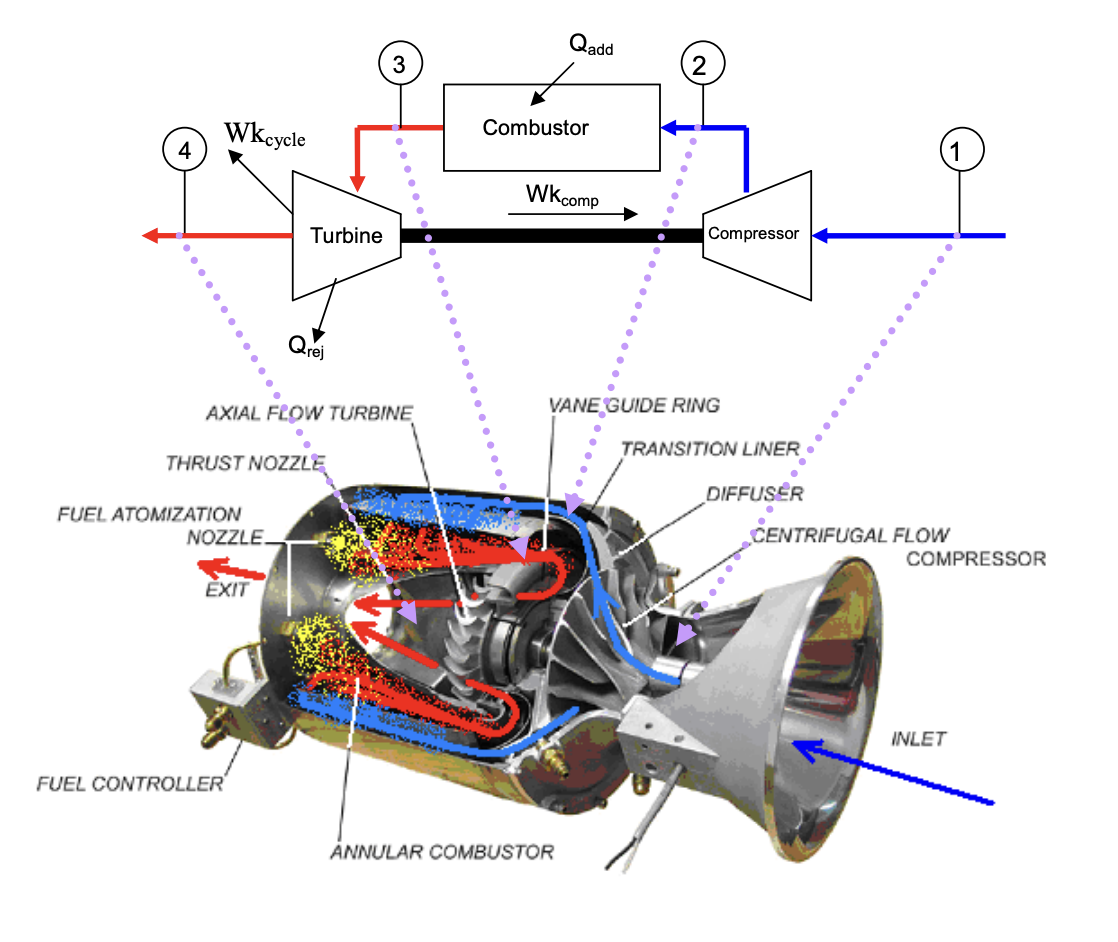
\includegraphics[keepaspectratio]{figuras/turbine_schema.png}}\end{minipage}%
\newline
\begin{minipage}{\linewidth}
Source: Mini-Lab Gas Turbine Power System Manual Turbine Technologies,
Ltd.
(\citeproc{ref-TurbineTechnologies2011MiniLab}{2011})\end{minipage}%

\end{figure}%

\subsection{Data Acquisition System and Control
Interface}\label{data-acquisition-system-and-control-interface}

The data acquisition process is managed through a dedicated Data
Acquisition Computer running the MiniLab 1.1 software. This computer
connects to the Mini-Lab system via a USB port, leveraging a National
Instruments DAQ (Data Acquisition) system (specifically the NI DAQ 6218
module) for real-time data capture and display. The MiniLab 1.1 software
facilitates logging data to file, displaying plot features, and offers
controls for unit toggling (e.g., Celsius to Fahrenheit for
temperatures, Psig to kPa for pressures, Liters/hour or Gallons/hour for
fuel flow, and Newtons to Pounds for thrust). The data sampling rate can
be selected between 0.1 and 5 samples per second.

\subsection{Experimental Procedure and Data Collection
Protocol}\label{experimental-procedure-and-data-collection-protocol}

The experimental procedure involved operating the Mini-Lab gas turbine
through its pre-start, start-up, and operational phases, followed by a
controlled shutdown. Prior to each run, essential checks were conducted,
including verification of fuel properties and ambient barometric
pressure \(P_{amb}=946.7 mbar\). During operation, the MiniLab 1.1
software collected real-time data from various sensors, including
temperatures, pressures, fuel flow, RPM, and thrust. This data was
logged continuously to a file on the connected computer's hard drive via
a USB connection to a National Instruments DAQ system. The software
allowed for adjustable sampling rates, and the recorded data was stored
in an ASCII format, enabling direct import into spreadsheet programs for
subsequent detailed analysis.

\section{\texorpdfstring{\textbf{Thermodynamic Modeling of the Gas
Turbine
System}}{Thermodynamic Modeling of the Gas Turbine System}}\label{thermodynamic-modeling-of-the-gas-turbine-system}

\subsection{System Overview}\label{system-overview}

The system of interest is a small-scale gas turbine engine operating in
steady-state. It consists of the following major components:

\begin{itemize}
    \item Compressor: Increases the pressure and temperature of incoming ambient air.
    \item Combustor: Mixes compressed air with fuel, where combustion raises the temperature significantly.
    \item Turbine: Extracts energy from the hot combustion gases to drive the compressor and generate useful work.
    \item Nozzle (Exhaust Section): Accelerates the exhaust gases to produce thrust.
\end{itemize}

Each component operates under the assumption of quasi-one-dimensional,
steady, adiabatic flow, with negligible heat loss to the surroundings
unless explicitly modeled.

\subsection{Assumptions and
Idealizations}\label{assumptions-and-idealizations}

To derive tractable analytical expressions and guide neural network
constraints, the following assumptions are adopted:

\begin{itemize}
    \item The working fluid (air and combustion gases) behaves as a calorically perfect ideal gas:
$$
    P = \rho R T, \quad c_p, c_v \text{ constant}, \quad \gamma = \frac{c_p}{c_v} \approx 1.4
$$

    \item Isentropic relations apply to ideal compression and expansion processes with specified efficiencies $\eta_c$ (compressor) and $\eta_t$ (turbine).
    \item Constant specific heats $c_p$ and $c_v$ are used, consistent with the assumption of ideal gases.
    \item No heat transfer or pressure losses in ducts, except where captured by model residuals.
    \item Steady-state and quasi-1D flow are assumed throughout.
\end{itemize}

\subsection{Key Thermodynamic
Equations}\label{key-thermodynamic-equations}

\subsubsection{Compressor}\label{compressor}

\begin{itemize}
    \item Isentropic temperature relation:
$$
    \frac{T_{2s}}{T_1} = \left( \frac{P_2}{P_1} \right)^{\frac{\gamma - 1}{\gamma}}
$$

    \item Actual outlet temperature considering efficiency:
$$
    T_2 = T_1 + \frac{T_{2s} - T_1}{\eta_c}
$$

    \item Power required by the compressor:
$$
    W_{\text{comp}} = \dot{m}_a c_p (T_2 - T_1)
$$

\end{itemize}

\subsubsection{Combustor}\label{combustor}

\begin{itemize}
    \item Energy balance (idealized with complete combustion and no heat losses):
$$
    \dot{m}_f Q_{\text{HV}} = (\dot{m}_a + \dot{m}_f) c_p (T_3 - T_2)
$$

    where $Q_{\text{HV}}$ is the lower heating value of the fuel and the gas mass flow is $\dot{m}_g = \dot{m}_a + \dot{m}_f$.
\end{itemize}

\subsubsection{Turbine}\label{turbine}

\begin{itemize}
    \item Isentropic temperature relation:
$$
    \frac{T_{4s}}{T_3} = \left( \frac{P_4}{P_3} \right)^{\frac{\gamma - 1}{\gamma}}
$$

    \item Actual outlet temperature considering turbine efficiency:
$$
    T_4 = T_3 - \eta_t (T_3 - T_{4s})
$$

    \item Power generated by the turbine:
$$
    W_{\text{turb}} = (\dot{m}_a + \dot{m}_f) c_p (T_3 - T_4)
$$

\end{itemize}

\subsubsection{Nozzle (Exhaust)}\label{nozzle-exhaust}

Assuming isentropic expansion and ambient back pressure \(P_0\), the
exhaust velocity is: \[
V_{\text{exit}} = \sqrt{2 c_p T_5 \left( 1 - \left( \frac{P_0}{P_5} \right)^{\frac{\gamma - 1}{\gamma}} \right)}
\]

The thrust is then calculated via momentum balance: \[
F = (\dot{m}_a + \dot{m}_f) (V_{\text{exit}} - V_{\text{inlet}})
\]

If inlet velocity is negligible (static tests), this simplifies to: \[
F \approx (\dot{m}_a + \dot{m}_f) V_{\text{exit}}
\]

\subsection{Station Numbering
Convention}\label{station-numbering-convention}

To standardize variables across the PINN and thermodynamic sections:

\begin{center}
\begin{tabular}{ll}
$1$ & Ambient conditions (inlet to compressor) \\
$2$ & Compressor exit / combustor inlet \\
$3$ & Combustor exit / turbine inlet \\
$4$ & Turbine exit / nozzle inlet \\
$5$ & Nozzle exit (exhaust gas temperature station)
\end{tabular}
\end{center}

This convention allows the PINN to learn both the observable outputs
(\(T_3\), \(T_5\), \(F\)) and intermediate station states (\(T_2\),
\(P_2\), \(T_4\), \(P_4\), etc.), constrained by physics-based
residuals.

\section{\texorpdfstring{\textbf{Physics-Informed Neural Network (PINN)
Framework}}{Physics-Informed Neural Network (PINN) Framework}}\label{physics-informed-neural-network-pinn-framework}

To bridge the gap between purely data-driven models and first-principle
simulations, this work employs a Physics-Informed Neural Network (PINN)
to model the gas turbine system.

\subsection{Core Concept}\label{core-concept}

PINNs are neural networks that embed physical laws directly into their
training process. Rather than minimizing only the error between model
predictions and experimental data, the PINN loss function also includes
terms that penalize violations of governing physical equations. This
approach ensures that predictions are both data-accurate and physically
consistent, even in regions where data is sparse.

\subsection{PINN Architecture}\label{pinn-architecture}

The core model is a fully connected Multi-Layer Perceptron (MLP) trained
to learn mappings from inputs to thermodynamic states and performance
metrics. The architecture is guided by simplifying assumptions from
thermodynamics:

\begin{itemize}
    \item Air is modeled as a calorically perfect ideal gas with constant specific heats ($c_p$, $c_v$) and a constant heat capacity ratio $\gamma = c_p / c_v \approx 1.4$.
    \item Isentropic efficiencies for the compressor ($\eta_c$) and turbine ($\eta_t$) are assumed constant.
    \item Heat losses, frictional effects, and pressure drops outside of defined station points are neglected.
\end{itemize}

Inputs: Key operational parameters that determine the thermodynamic
state of the system:

\begin{itemize}
    \item Fuel flow rate $\dot{m}_f$ ($\mathrm{kg/s}$)
    \item Compressor rotational speed $N_1$ (RPM)
    \item Ambient temperature $T_1$ (K)
    \item Ambient pressure $P_1$ (Pa)
\end{itemize}

Outputs: Predicted thermodynamic variables and performance indicators:

\begin{itemize}
    \item Station states: $T_{2,\text{pred}}, P_{2,\text{pred}}, T_{3,\text{pred}}, P_{3,\text{pred}}, T_{4,\text{pred}}, P_{4,\text{pred}}, T_{5,\text{pred}}, P_{5,\text{pred}}$
    \item Net thrust $F_{\text{pred}}$ (N)
    \item Air mass flow rate $\dot{m}_{a, \text{pred}}$ (kg/s)
\end{itemize}

\subsection{Hybrid Loss Function}\label{hybrid-loss-function}

The total loss used to train the PINN is a weighted sum of data-driven
and physics-based components: \[
L_{\text{total}} = w_{\text{data}} L_{\text{data}} + w_{\text{physics}} L_{\text{physics}}
\]

\begin{itemize}
    \item Data Loss ($L_{\text{data}}$): A supervised learning loss (Mean Squared Error) that penalizes deviation from available experimental measurements:
$$
    L_{\text{data}} = \frac{1}{N} \sum_{i=1}^{N} \left( y_i - y_{i,\text{pred}} \right)^2
$$
    
    \item Physics Loss ($L_{\text{physics}}$): A sum of residuals derived from physical principles, each enforcing thermodynamic consistency.
\end{itemize}

\subsubsection{\texorpdfstring{Compressor Temperature Rise Loss
(\(L_{T2}\))}{Compressor Temperature Rise Loss (L\_\{T2\})}}\label{compressor-temperature-rise-loss-l_t2}

Derived from the isentropic temperature relation: \[
L_{T2} = \left( \eta_c (T_{2,\text{pred}} - T_1) - T_1 \left( \left(\frac{P_{2,\text{pred}}}{P_1}\right)^{\frac{\gamma-1}{\gamma}} - 1 \right) \right)^2
\]

\subsubsection{\texorpdfstring{Turbine Temperature Drop Loss
(\(L_{T4}\))}{Turbine Temperature Drop Loss (L\_\{T4\})}}\label{turbine-temperature-drop-loss-l_t4}

Enforcing the relationship between pressure drop and temperature drop
across the turbine: \[
L_{T4} = \left( (T_{3,\text{pred}} - T_{4,\text{pred}}) - \eta_t T_{3,\text{pred}} \left(1 - \left(\frac{P_{4,\text{pred}}}{P_{3,\text{pred}}}\right)^{\frac{\gamma-1}{\gamma}}\right) \right)^2
\]

\subsubsection{\texorpdfstring{Shaft Power Balance Loss
(\(L_{\text{power}}\))}{Shaft Power Balance Loss (L\_\{\textbackslash text\{power\}\})}}\label{shaft-power-balance-loss-l_textpower}

For a single-shaft turbojet, the power generated by the turbine
(\(W_{\text{turb}}\)) is consumed entirely by the compressor
(\(W_{\text{comp}}\)). This constraint,
\(W_{\text{turb}} = W_{\text{comp}}\), provides a fundamental physical
link between the component states. The loss residual enforces this
balance. \[
L_{\text{power}} = \left( (\dot{m}_a + \dot{m}_f) c_p (T_{3,\text{pred}} - T_{4,\text{pred}}) - \dot{m}_a c_p (T_{2,\text{pred}} - T_1) \right)^2
\]

\subsubsection{\texorpdfstring{Combustor Energy Balance Loss
(\(L_{\text{comb}}\))}{Combustor Energy Balance Loss (L\_\{\textbackslash text\{comb\}\})}}\label{combustor-energy-balance-loss-l_textcomb}

Assuming ideal heat release with no losses: \[
L_{\text{comb}} = \left( \dot{m}_f Q_{\text{HV}} - (\dot{m}_a + \dot{m}_f) c_p (T_{3,\text{pred}} - T_{2,\text{pred}}) \right)^2
\]

\subsubsection{Thrust Loss}\label{thrust-loss}

A simplified thrust estimation (using momentum conservation) could also
be encoded if exit velocity and intake velocity are known or modeled: \[
L_{\text{thrust}} = \left( F_{\text{pred}} - (\dot{m}_a + \dot{m}_f) (V_{\text{exit}}) \right)^2
\]

While air mass flow rate \(\dot{m}_a\) could be derived from a
physics-based model based on \(N_1\) and ambient conditions, in this
PINN-based approach, it is treated as a learnable parameter. This allows
the model to infer the air mass flow rate directly from the operational
data, providing a more flexible and potentially more accurate estimation
by capturing complex relationships that a simplified physics model might
overlook.

\section{\texorpdfstring{\textbf{Model Implementation and
Evaluation}}{Model Implementation and Evaluation}}\label{model-implementation-and-evaluation}

This section outlines the strategy for the development, training, and
rigorous evaluation of the gas turbine digital twin.

\subsection{Problem Definition}\label{problem-definition}

The primary objective is to develop a digital twin capable of predicting
key performance indicators---steady-state thrust (\(F_{pred}\)),
combustor outlet temperature (\(T_{3,pred}\)), and exhaust gas
temperature (\(T_{5,pred}\))---based on operational inputs (fuel flow
\(\dot{m}_f\), compressor speed \(N_1\)) and ambient conditions
(\(T_1, P_1\)).

To enforce physical realism, the model simultaneously predicts a set of
intermediate thermodynamic variables: - Air mass flow:
\(\dot{m}_{a,pred}\) - Station temperatures: \(T_{2,pred}, T_{4,pred}\)
- Station pressures: \(P_{2,pred}, P_{3,pred}, P_{4,pred}, P_{5,pred}\)

These intermediate predictions are constrained during training by the
physics-informed loss functions derived in the previous chapter.

\subsection{Data Preparation and
Preprocessing}\label{data-preparation-and-preprocessing}

The experimental dataset undergoes a standard preprocessing pipeline
before being used for model training:

\begin{itemize}
\tightlist
\item
  Unit Conversion: All variables are converted to base SI units (e.g.,
  temperatures to Kelvin, pressures to Pascals, fuel flow to kg/s) to
  ensure consistency in the physics-based calculations.
\item
  Normalization: Input and output features are scaled to a common range
  (e.g., {[}0, 1{]}) using min-max scaling. This improves numerical
  stability during training and helps the optimization algorithm
  converge more efficiently.
\item
  Data Splitting: The complete dataset is randomly partitioned into
  three subsets: 80\% for training, 10\% for validation (hyperparameter
  tuning), and 10\% for final, unbiased testing of the trained model.
\end{itemize}

\subsection{Model Architecture and
Hyperparameters}\label{model-architecture-and-hyperparameters}

The core of the digital twin is a Physics-Informed Neural Network (PINN)
based on a Multi-Layer Perceptron (MLP).

\begin{itemize}
\tightlist
\item
  Baseline Architecture: The initial architecture for exploration is a
  fully connected MLP with 4 input neurons, 2 hidden layers containing
  32 neurons each, and 10 output neurons.
\item
  Inputs (4): Fuel flow (\(\dot{m}_f\)), compressor speed (\(N_1\)),
  ambient temperature (\(T_1\)), and ambient pressure (\(P_1\)).
\item
  Outputs (10): Thrust (\(F_{pred}\)), air mass flow
  (\(\dot{m}_{a,pred}\)), and the eight station states
  (\(T_{2,pred}, P_{2,pred}, T_{3,pred}, P_{3,pred}, T_{4,pred}, P_{4,pred}, T_{5,pred}, P_{5,pred}\)).
\item
  Activation Functions: The ReLU (Rectified Linear Unit) activation
  function is used for hidden layers, while a Linear activation is used
  for the output layer to allow for unbounded physical values.
\item
  Hyperparameter Tuning: A hyperparameter search will be conducted using
  the validation set to optimize the network architecture (e.g., number
  of layers and neurons), learning rate, and loss function weights to
  achieve the best performance. The search will be using a random search
  with 10 iterations.
\end{itemize}

\subsection{Loss Function and Weighting
Strategy}\label{loss-function-and-weighting-strategy}

The custom loss function guides the PINN to be both data-accurate and
physically-consistent. The total loss is a weighted sum of two
components: \[
L_{total} = w_{data} L_{data} + w_{physics} L_{physics}
\]

\begin{itemize}
\tightlist
\item
  Data Loss (\(L_{data}\)): This is the Mean Squared Error (MSE) between
  the model's predictions and the measured experimental data for the
  observable outputs (\(T_3, T_5, F\), etc.).
\item
  Physics Loss (\(L_{physics}\)): This is the sum of the mean squared
  residuals from the governing thermodynamic equations (e.g.,
  \(L_{power}, L_{comb}, L_{T2}, L_{T4}\)). This term penalizes
  solutions that violate physical laws.
\item
  Weighting Strategy: The weights (\(w_{data}, w_{physics}\)) are
  critical hyperparameters that balance the influence of the
  experimental data and the physical laws. A sensitivity analysis will
  be performed to find a set of weights that minimizes prediction error
  on the validation set without compromising physical consistency.
\end{itemize}

\subsection{Training and Evaluation
Metrics}\label{training-and-evaluation-metrics}

The model will be implemented and trained using the PyTorch framework
with the AdamW optimizer. To ensure a thorough and unbiased assessment
of the final digital twin, its performance will be evaluated on the
unseen test set using three key criteria:

\begin{enumerate}
\def\labelenumi{\arabic{enumi}.}
\tightlist
\item
  \textbf{Predictive Accuracy:} The model's ability to predict the
  primary performance indicators will be quantified using Mean Squared
  Error (MSE) for \(F_{pred}\), \(T_{3,pred}\), and \(T_{5,pred}\).
\item
  \textbf{Physical Consistency:} The magnitude of the physics loss
  residuals (\(L_{physics}\)) will be calculated on the test set. A low
  residual value indicates that the model's predictions adhere well to
  the governing laws of thermodynamics, even for data it has never seen.
\item
  \textbf{Overall Fidelity:} The accuracy of the intermediate variable
  predictions (e.g., \(P_2, T_2, \dot{m}_a\)) will also be assessed to
  ensure the overall health and internal consistency of the model.
\end{enumerate}

\backmatter

\newpage
\chapter*{\textbf{Bibliography}}
\markboth{BIBLIOGRAPHY}{BIBLIOGRAPHY}

\phantomsection\label{refs}
\begin{CSLReferences}{0}{1}
\bibitem[\citeproctext]{ref-boyce2012gasturbine}
BOYCE, Meherwan P. \textbf{Gas Turbine Engineering Handbook}.
\emph{{[}S.l.{]}}: Elsevier Science, 2012.

\bibitem[\citeproctext]{ref-cengel2019thermodynamics}
CENGEL, Yunus A.; BOLES, Michael A. \textbf{Thermodynamics: An
Engineering Approach}. \emph{{[}S.l.{]}}: McGraw-Hill Education, 2019.

\bibitem[\citeproctext]{ref-goodfellow2016deep}
GOODFELLOW, Ian; BENGIO, Yoshua; COURVILLE, Aaron. \textbf{Deep
Learning}. \emph{{[}S.l.{]}}: MIT Press, 2016.

\bibitem[\citeproctext]{ref-grieves2011digital}
GRIEVES, Michael. Digital Twin: Manufacturing Excellence through Virtual
Replica of Physical Product for Future Factory. \textbf{White Paper,
Florida Institute of Technology}, 2011.

\bibitem[\citeproctext]{ref-gurney2010gasturbine}
GURNEY, L. S. \textbf{Gas Turbine Performance}. \emph{{[}S.l.{]}}:
Butterworth-Heinemann, 2010.

\bibitem[\citeproctext]{ref-incropera2007fundamentals}
INCROPERA, Frank P. \emph{et al.} \textbf{Fundamentals of Heat and Mass
Transfer}. \emph{{[}S.l.{]}}: John Wiley \& Sons, 2007.

\bibitem[\citeproctext]{ref-karniadakis2021physics}
KARNIADAKIS, George Em \emph{et al.} Physics-informed machine learning.
\textbf{Nature Reviews Physics}, v. 3, n. 6, p. 422--441, 2021.

\bibitem[\citeproctext]{ref-kreuzer2024artificial}
KREUZER, Tim; PAPAPETROU, Panagiotis; ZDRAVKOVIC, Jelena. Artificial
intelligence in digital twins---A systematic literature review.
\textbf{Data \& Knowledge Engineering}, 2024.

\bibitem[\citeproctext]{ref-kurz2009gasturbine}
KURZ, R.; BRUN, K. \textbf{Gas Turbine System Design, Analysis, and
Optimization}. \emph{{[}S.l.{]}}: ASME Press, 2009.

\bibitem[\citeproctext]{ref-raissi2019physics}
RAISSI, Maziar; PERDIKARIS, Paris; KARNIADAKIS, George E.
Physics-informed neural networks: A deep learning framework for solving
forward and inverse problems involving nonlinear partial differential
equations. \textbf{Journal of Computational Physics}, v. 378, p.
686--707, 2019.

\bibitem[\citeproctext]{ref-russell2010artificial}
RUSSELL, Stuart; NORVIG, Peter. \textbf{Artificial Intelligence: A
Modern Approach}. \emph{{[}S.l.{]}}: Prentice Hall, 2010.

\bibitem[\citeproctext]{ref-saravanamuttoo2017gasturbine}
SARAVANAMUTTOO, H. I. H. \emph{et al.} \textbf{Gas Turbine Theory}.
\emph{{[}S.l.{]}}: Pearson, 2017.

\bibitem[\citeproctext]{ref-schluse2018digital}
SCHLUSE, Martin \emph{et al.} Digital Twin: An Overview of the Current
State. \emph{In}: \textbf{Virtual and Augmented Reality in Industry}.
\emph{{[}S.l.{]}}: Springer, Cham, 2018. p. 253--272.

\bibitem[\citeproctext]{ref-serway2018physics}
SERWAY, Raymond A.; JEWETT, John W. \textbf{Physics for Scientists and
Engineers with Modern Physics}. \emph{{[}S.l.{]}}: Cengage Learning,
2018.

\bibitem[\citeproctext]{ref-tao2019digital}
TAO, Fei \emph{et al.} \textbf{Digital Twin Driven Smart Manufacturing}.
\emph{{[}S.l.{]}}: Elsevier, 2019.

\bibitem[\citeproctext]{ref-TurbineTechnologies2011MiniLab}
TURBINE TECHNOLOGIES, LTD. \textbf{Mini-Lab Gas Turbine Power
System{\texttrademark} Sample Lab Experiment Manual}. \emph{{[}S.l.{]}}:
Turbine Technologies, Ltd., 2011.

\bibitem[\citeproctext]{ref-verstraete2010cfd}
VERSTRAETE, D.; VAN DEN BRAEMBUSSCHE, R. A. \textbf{CFD for
Turbomachinery}. \emph{{[}S.l.{]}}: VKI Lecture Series, 2010.

\bibitem[\citeproctext]{ref-wang2023physics}
WANG, Yibin; LU, Beijia; ZHANG, Jian. A physics-informed neural network
for modeling and prognosis of steam turbine performance. \textbf{Applied
Thermal Engineering}, v. 223, p. 119934, 2023.

\end{CSLReferences}




\end{document}
